%%% TokenSmith 3-minute class presentation
%%% Compile with pdflatex (Beamer). Aspect ratio 16:9.

\documentclass[aspectratio=169,11pt]{beamer}

\usetheme{Madrid}
\usecolortheme{seahorse}
\setbeamertemplate{navigation symbols}{}
\setbeamertemplate{footline}[frame number]

\usepackage{tikz}
\usetikzlibrary{positioning, arrows.meta}
\usepackage{booktabs}
\usepackage{graphicx}

\title[TokenSmith on Consumer GPUs]{Optimizing TokenSmith for Consumer-GPU Hardware}
\subtitle{A Local-First RAG Pipeline}
\author{Shivam Singhal}
\institute{Georgia Tech}
\date{CS 6423, Spring 2026}

\begin{document}

%% ----------------------------------------------------------
\begin{frame}
  \titlepage
\end{frame}

%% ----------------------------------------------------------
\begin{frame}{The problem}
TokenSmith is a local-first RAG system for textbook question answering.
No external API calls, everything runs on the student's machine.

\bigskip

The original system works, but the cold path is brutal:
\begin{itemize}
  \item Sequential PDF extraction: \textbf{9{,}650\,s} (about 2h 40m)
  \item 4\,B embedder build: another 5 to 7 minutes on a server GPU
  \item First answer: a few seconds, after all of that
\end{itemize}

\bigskip

\begin{block}{}
\centering
\textbf{Cold time-to-first-token on a laptop: $\sim$\,2h 45m.}\\
Nobody waits that long for one textbook.
\end{block}
\end{frame}

%% ----------------------------------------------------------
\begin{frame}{The pipeline and where we attacked it}
\centering
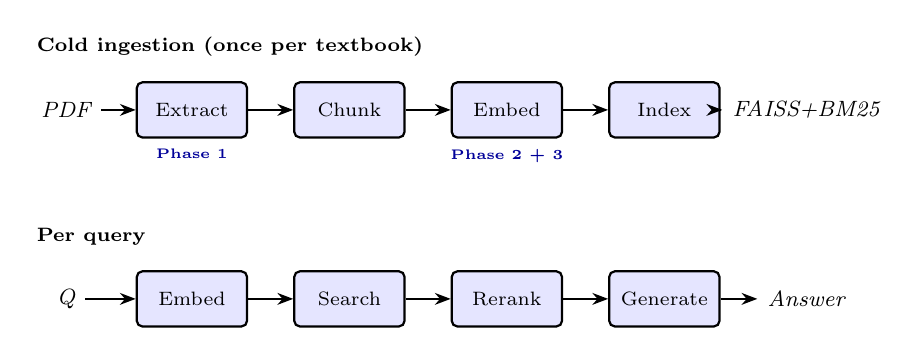
\begin{tikzpicture}[
  > = {Stealth[length=2mm]},
  thick,
  font=\scriptsize,
  stage/.style={draw, rounded corners=2pt, fill=blue!10,
                minimum width=14mm, minimum height=7mm, align=center},
  io/.style={font=\footnotesize\itshape},
  arr/.style={->, thick}
]
  \node[io]    (pdf) at (0, 0)   {PDF};
  \node[stage] (ext) at (1.6, 0) {Extract};
  \node[stage] (chk) at (3.6, 0) {Chunk};
  \node[stage] (emb) at (5.6, 0) {Embed};
  \node[stage] (idx) at (7.6, 0) {Index};
  \node[io]    (db)  at (9.4, 0) {FAISS+BM25};

  \draw[arr] (pdf) -- (ext);
  \draw[arr] (ext) -- (chk);
  \draw[arr] (chk) -- (emb);
  \draw[arr] (emb) -- (idx);
  \draw[arr] (idx) -- (db);

  \node[anchor=north, font=\tiny\bfseries, color=blue!60!black]
    at (ext.south) {Phase 1};
  \node[anchor=north, font=\tiny\bfseries, color=blue!60!black]
    at (emb.south) {Phase 2 + 3};
  \node[anchor=south west, font=\scriptsize\bfseries]
    at (-0.5, 0.55) {Cold ingestion (once per textbook)};

  \node[io]    (q)   at (0, -2.4)   {Q};
  \node[stage] (qe)  at (1.6, -2.4) {Embed};
  \node[stage] (sr)  at (3.6, -2.4) {Search};
  \node[stage] (rer) at (5.6, -2.4) {Rerank};
  \node[stage] (gen) at (7.6, -2.4) {Generate};
  \node[io]    (a)   at (9.4, -2.4) {Answer};

  \draw[arr] (q)   -- (qe);
  \draw[arr] (qe)  -- (sr);
  \draw[arr] (sr)  -- (rer);
  \draw[arr] (rer) -- (gen);
  \draw[arr] (gen) -- (a);

  \node[anchor=south west, font=\scriptsize\bfseries]
    at (-0.5, -1.85) {Per query};
\end{tikzpicture}

\vspace{1ex}
\small
\textbf{Phase 1:} faster PDF extraction.
\textbf{Phase 2:} hardware-aware embedding.
\textbf{Phase 3:} pluggable embedder backends.

\note{Cold path runs once per textbook, per-query path runs every
question. Phases 1, 2, 3 all touch the cold path.}
\end{frame}

%% ----------------------------------------------------------
\begin{frame}{Phase 1 v1: parallelize PDF extraction}
Layout analysis dominates \texttt{docling}; it runs page-by-page and
the pages are independent. Restructure as map-reduce: split the PDF,
run \texttt{docling} workers in parallel, reduce on offset.

\begin{columns}[T,onlytextwidth]
\begin{column}{0.42\textwidth}
\centering
\footnotesize
\begin{tabular}{rrr}
\toprule
workers & wall (s) & speedup \\
\midrule
1   & 9{,}650 & 1.0$\times$ \\
4   & 2{,}018 & 4.8$\times$ \\
16  & 1{,}116 & 8.7$\times$ \\
32  & 535     & 18.0$\times$ \\
62  & 382     & \textbf{25.3$\times$} \\
\bottomrule
\end{tabular}
\end{column}
\begin{column}{0.55\textwidth}
\centering
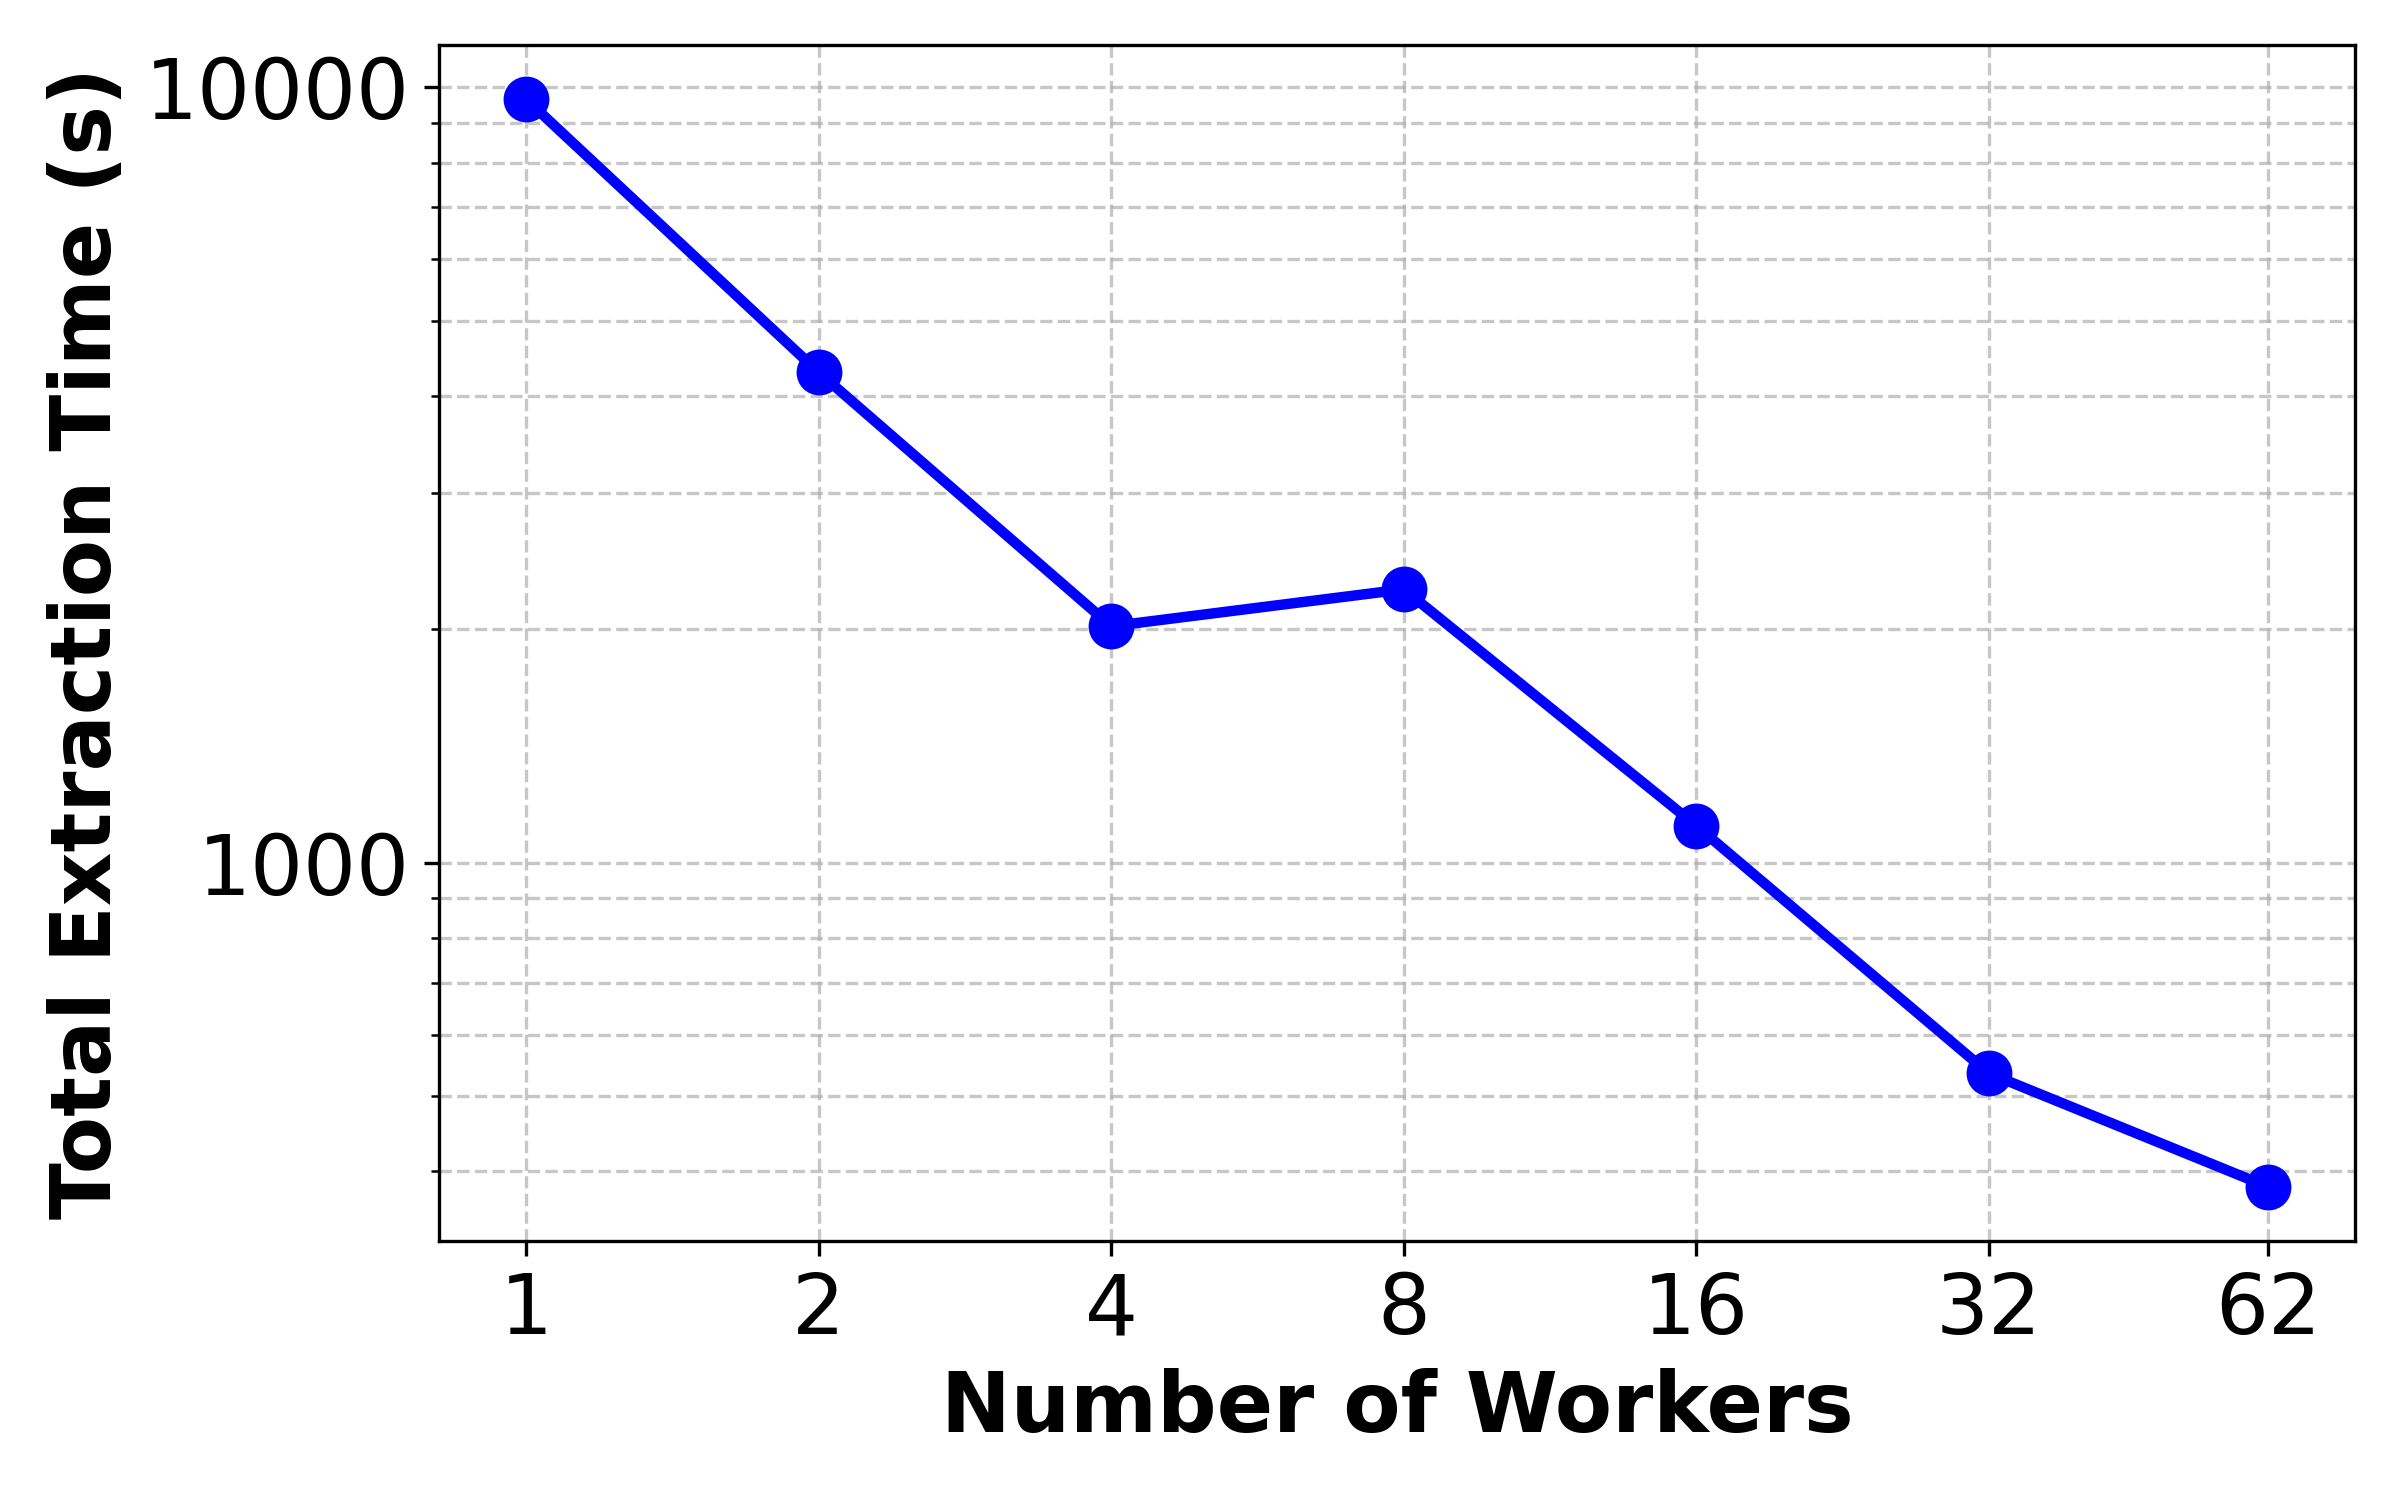
\includegraphics[width=\linewidth]{figs/extraction_scaling.png}
\end{column}
\end{columns}

\vspace{0.5ex}
\begin{block}{}
\centering
\textbf{25.3$\times$ speedup at 62 workers.} A consumer laptop has
4 cores, not 62, and 4 workers still takes $\sim$\,34 minutes.
Parallelism alone does not get us there.
\end{block}

\note{The scaling is real on a server. The 8-worker dip is a small
cache-pressure artifact at the chosen chunk size. The point of the
slide: even with this win, a 4-core laptop is stuck at 34 minutes.}
\end{frame}

%% ----------------------------------------------------------
\begin{frame}{Phase 1 v2: pypdfium2 fast path}
Plain-text textbooks do not need layout analysis. Skip \texttt{docling}
entirely. Use \texttt{pypdfium2} to read raw text directly from each
page range; recover section headings with a regex on
``\texttt{N.N Title}'' patterns.

\bigskip

\begin{block}{}
\centering
\textbf{2h 40m $\rightarrow$ 8.66\,s} (4 workers, RTX 6000 host).
\\[0.4ex]
$\sim$\,$\mathbf{1{,}100\times}$ faster than the original sequential
\texttt{docling} extractor.
\end{block}

\bigskip

\begin{columns}[T,onlytextwidth]
\begin{column}{0.48\textwidth}
\textbf{Pros}
\begin{itemize}
  \item $\sim$\,1{,}100$\times$ faster on the textbook
  \item No temp files, no map-phase split
  \item End-to-end answer quality slightly \emph{better}
        (final 0.606 vs 0.592)
\end{itemize}
\end{column}
\begin{column}{0.48\textwidth}
\textbf{Cons}
\begin{itemize}
  \item No layout analysis
  \item Tables, multi-column papers, scanned PDFs need
        \texttt{docling}
  \item Regex heading detection is fragile on non-standard layouts
\end{itemize}
\end{column}
\end{columns}

\note{For the textbook target, layout analysis was overhead. We keep
docling available for documents that genuinely need it.}
\end{frame}

%% ----------------------------------------------------------
\begin{frame}{Phase 2: hardware router and length-sorted batches}
Two small fixes inside the embedder.

\bigskip

\textbf{Problem 1.} The indexer always used a CPU process pool, even
when a GPU was reachable. The pool fights the GPU's allocator on
mixed hosts.\\
\textbf{Fix.} Detect the GPU at startup; pick sequential GPU vs CPU
pool accordingly.

\bigskip

\textbf{Problem 2.} \texttt{llama.cpp} pads each embedding batch to the
longest text in that batch. Random ordering wastes compute on short
texts that share a batch with one long text.\\
\textbf{Fix.} Sort inputs by length descending before batching, and
permute the result back so the FAISS index ID order is unchanged.

\note{Don't dwell on this slide. Two small wins in the embedder.}
\end{frame}

%% ----------------------------------------------------------
\begin{frame}{Phase 3: pluggable embedder backends}
\textbf{Motivation.} A 4\,B embedder is heavy. Can a 23\,M model match
its answer quality on a small corpus?

\medskip

\textbf{Approach.} Refactor the embedder around a backend interface.
One keyword argument switches between \texttt{llama.cpp} (4\,B GGUF),
GPT4All (Vulkan or CUDA), and HuggingFace
\texttt{sentence-transformers} (Nomic-v1.5 137\,M, MiniLM 23\,M).

\medskip

\centering
\footnotesize
\begin{tabular}{lrrr}
\toprule
variant            & params  & peak VRAM  & final \\
\midrule
4\,B baseline (llama.cpp) & 4\,B    & 5.4\,GiB   & 0.592 \\
\textbf{MiniLM (HF)}      & 23\,M   & 2.2\,GiB   & \textbf{0.578} \\
Nomic (HF)                & 137\,M  & 2.7\,GiB   & 0.563 \\
Nomic (GPT4All Vulkan)    & 137\,M  & 2.1\,GiB   & 0.558 \\
\bottomrule
\end{tabular}

\vspace{1ex}
\begin{block}{}
\centering
\textbf{Cold time-to-first-token: $\sim$\,2h 48m $\rightarrow$
$\sim$\,45 s} on a 4-core / 8\,GiB consumer GPU. Over 200$\times$.
\\[0.4ex]
MiniLM matches the 4\,B baseline within 1.4 points on final score.
\end{block}

\note{Headline number first: 200x speedup. Then the table. Then the
quality story: a 23M model is enough on this corpus.}
\end{frame}

%% ----------------------------------------------------------
\begin{frame}{Takeaways}
\begin{itemize}
  \item For plain-text textbooks, layout-aware PDF extraction was
    overkill. \texttt{pypdfium2} is roughly 1{,}100$\times$ faster
    than the original sequential \texttt{docling} and slightly
    \emph{better} on end-to-end answer quality.
  \medskip
  \item On a small corpus, the cross-encoder reranker absorbs the
    embedding-quality gap. A 23\,M MiniLM matches a 4\,B model on
    final answer quality, because the right chunk only has to land in
    the FAISS top-50 for the reranker to find it.
  \medskip
  \item TokenSmith now runs end to end on a 4-core / 8\,GiB consumer
    machine. The remaining latency floor is cold extraction, which we
    drove to 8.66\,s on the textbook.
\end{itemize}

\bigskip
\centering
\small
Code: \texttt{github.com/singhals163/TokenSmith}

\note{End on the cross-encoder insight. The story is not about
inventing new tricks; it's about removing the parts that do not earn
their cost.}
\end{frame}

%% ----------------------------------------------------------
\begin{frame}
  \centering
  {\Huge Questions?}\\[2em]
  \small \texttt{github.com/singhals163/TokenSmith}
\end{frame}

\end{document}
